\section{Hardware}

\subsection{Motor und Controller}\label{subsec:MotorController}
Gemäss den Anforderungen an das Projekt, soll die gesamte Ansteuerung im Kleinspannungsbereich realisiert und mit Batterien versorgt werden. Diese liegt gemäss IEC 60449 Norm bei Gleichspannung $120V_{DC}$ und Wechselspannung $50V_{AC}$. Um einen Gleitschirmpiloten in die Luft zu heben, muss der Motor auch über ein grosses Drehmoment und genügend Leistung verfügen. Aus der Literatur Gleitsegelschlepp \cite{Gleitsegelschlepp} ist ersichtlich, dass der Gleitschirmpilot mit bis zu 10m/s gezogen wird. Aus den Richtlinien, welche der deutsche Gleitschirmverband erlassen hat, ist wiederrum ersichtlich, dass mit einer Zugkraft von bis zu 1kN bei Solopiloten und 1,3kN bei Tandempiloten gezogen werden darf \cite{WindenProtokoll} (Punkt 24). Daraus lässt sich die maximale Leistung, welche das System auf den Gleitschirmpiloten ausüben darf ausrechnen [Referenz auf irgend ein Physikbuch]:


\begin{equation}
\centering
P_{Seil}=F \cdot \nu=1300N \cdot 10m/s=13kW
\label{eq:LeistungSeil}
\end{equation}

Da es sich um ein reales System handelt und deswegen im Motor, in Übertragung und Übersetzung Verluste auftreten, wird für die erste Handrechnung mit einem Gesamtwirkungsgrad des Systems von 80$\%$ gerechnet.

\begin{equation}
\centering
P_{Motor}==\frac{P_{Seil}}{\eta}=\frac{13kW}{0.8}=16.3kW
\label{eq:LeistungMotor}
\end{equation}

Da diese Leistung nicht über einen längeren Zeitraum geleistet werden muss, darf der Motor leicht unterdimensioniert werden. Als Realisierungsmöglichkeiten standen somit lediglich Wechselstrommotoren mit Wechselrichter, DC-Motoren oder Brushless DC (auch BLDC) Motoren in Frage kommen. Nachfolgend ist eine Auswahl an Motoren mit deren Controller aufgelistet.

\begin{figure}[H]
	\begin{center}
		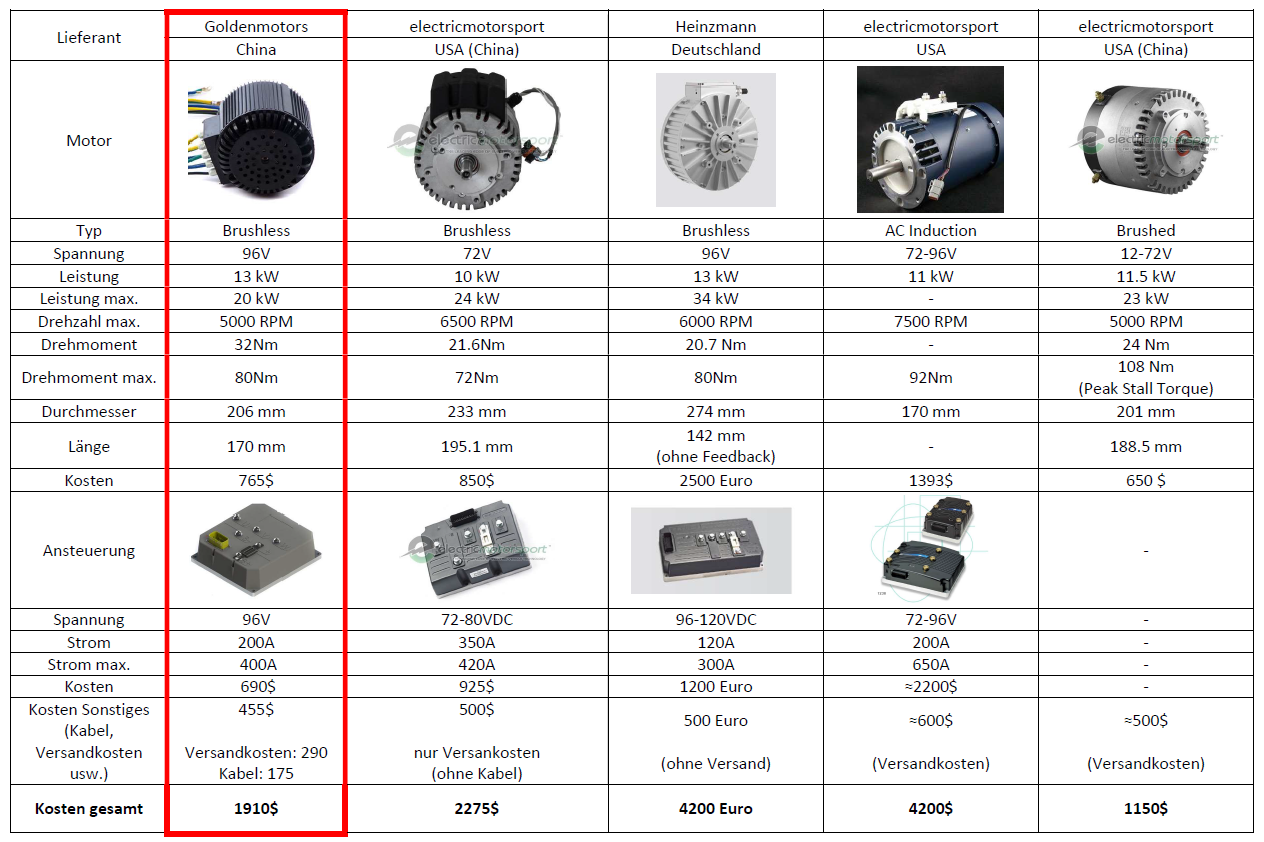
\includegraphics[width=160mm]{motor.png}
		\caption[Motorenvergleich]{Motor} %picture caption
		\label{fig:Motorenvergleich}
	\end{center}
\end{figure}

ES FOLGT TEXT ZU: WESHALB DIESER MOTOR AUSGEWÄHLT WURDE


Ausserdem wurde beim Motor die 96V Variante ausgewählt, da dieser durch die erhöhte Spannung einen kleineren Strom benötigt. Dadurch können kleinere Querschnitte gefahren werden, wodruch an Material eingespart werden kann.

\subsection{Energieversorgung}\label{subsec:Energieversorgung}

Damit die Einzugswinde betrieben werden kann, wird das gesamte System von einer Batterie gespiessen. Wie im vorhergehenden Abschnitt \ref{subsec:MotorController} beschrieben, wurde ein Motor mit 96V Nennspannung ausgewählt. Aus diesem Grund ist es notwendig, Batterien mit derselben Versorgungsspannung zu verwenden. Durch die fortlaufende Weiterentwicklung von Akkumulatoren, stellte sich die Frage nach dem Typ und der notwendigen Kapazität für den Betrieb. Trotz der steilen Entwicklungskurve von Li-Ionen Akkus, sind sie im Vergleich zu kommerziellen Blei-Akkus, komplizierter und heikler in der Handhabung (Ladeschaltung mit Zellenüberwachung notwendig) und vor allem teurer. Es muss jedoch berücksichtigt werden, dass auch bei Bleiakkus zwischen zwei Typen unterschieden wird. Zum einen werden oft Starterbatterien (hohe Anlaufströme, kurze Laufzeit) verwendet, und zum anderen zyklenfeste Bleiakkumulatoren (lange Laufzeit, ausgelegt für viele Lade-/ Entladevorgänge). Es ist klar ersichtlich, dass die zyklenfesten Modelle besser in den Versorgungsbetrieb unseres Projektes passen, jedoch muss bedenkt werden, dass sie durch die hohe Zyklenfestigkeit auch wesentlich teurer sind als die anderen. Um einen Überblick zu erhalten, befinden sich im Anhang (\ref{appsec:Batterie}) zwei Tabellen mit einigen Modellen von jedem Typen. Diese werden jeweils in den elektrischen Klassifizierungen (Typ, Spannung, Kapazität), wie auch weiteren Merkmalen (wie Gewicht, Preis, Anzahl Starts) mit einander verglichen. Die Zyklenfesten Batterien wurden zusätzlich mit der vom Hersteller Angegebenen Zyklenfestigkeit und den jeweiligen Innenwiderständen ergänzt. Der Innenwiderstand wurde zusätzlich als wichtig betrachtet, da bei hohen Strömen (gemäss dem Ohmschen Gesetz) eine Spannung über den Batterien abfällt. Daher gilt: Umso grösser der Innenwiderstand, desto grösser die abfallende Spannung über den Batterien, wodurch eine kleinere Spannung an den Motor gelangt.
Damit man ein Gefühl für die Grössenordnung der jeweiligen Kapazitäten erhält, wurden die Anzahl möglichen Starts berechnet. Dafür wurden zuerst einige Annahmen getroffen.

\begin{table}[H]
	\centering
	\begin{tabular}{C{5cm} C{2.5cm} C{2cm}}
		\multicolumn{3}{c}{}}\\
		{Beschreibung} & {Index} & {Wert} \\ \hline
		Zugkraft    &   $ F_{Zug} $    & $10 kN$   \\
		Geschwindigkeit    &   $ v $    & $10 m/s$   \\
		Startzeit    &   $ t $   & $120 s$   \\
		Gesamtwirkungsgrad    &  $ \eta_{tot} $    & $80\%$   \\
		Auslastung    &  $ \theta $   & $80\%$  \\
		Batterieausnutzung    &  $ \kappa $    & $60\%$   \\
		Energie    &   $ W $    &   \\
		Anzahl Starts    &   $ n $    &    \\	
\end{tabular}
	\caption{Annahmen für Berechnung}
	\label{tab:BerechnungAnzahlStart}
\end{table}


Die Modelle mit dem besten Preis-Leistungsverhältnis wurden grün hervorgehoben. Diese entsprechen jedoch nicht unbedingt der günstigsten Variante.
